\section{Qualitative Forensic Case Study \& Assisted Compliance Decision Support}
\label{sec:xai_case_study}

\subsection{15-Node Fan-In \& Peeling Chain Model Attribution}
\label{sec:xai_attribution}

\begin{figure}[pos=tb]
\centering
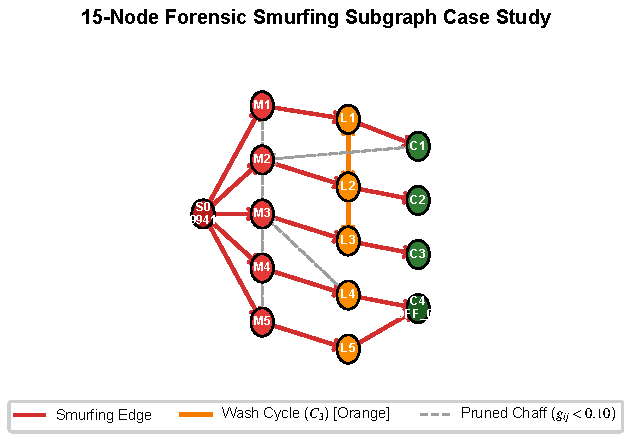
\includegraphics[width=\columnwidth]{figures/15_node_subgraph.pdf}
\caption{Qualitative Attribution: 15-node Bitcoin Elliptic transaction subgraph via GNNExplainer \citep{ying2019gnnexplainer}. Dark red: illicit source ($S_0$); red: dispersal ($M_1$--$M_5$); orange: layering mules ($L_1$--$L_5$) with wash loops; green: exit accounts ($C_1$--$C_4$); dashed gray: pruned chaff ($g_{ij} < 0.10$). Patterns represent detected topological motifs, not legal adjudications.}
\label{fig:causal_subgraph}
\end{figure}
To evaluate model interpretability under regulatory auditability standards, we examine an illustrative money-laundering smurfing campaign reconstructed from verified typological subgraphs (Fig.~\ref{fig:causal_subgraph}) as an illustrative, qualitative attribution study designed to inspect feature and topological saliency rather than establish legal adjudication. Saliency weights from GNNExplainer \citep{ying2019gnnexplainer} reveal four distinct operational stages:
\begin{enumerate}
    \item \textit{Dispersal ($S_0 \to M_{1\dots 5}$):} $S_0$ distributes \$48,500 across five accounts in sub-\$10,000 bursts over 22 minutes (characteristic structuring below the statutory \$10,000 currency reporting threshold under 31 U.S.C. \S~5324 and the Bank Secrecy Act);
    \item \textit{Layering ($M \to L_{1\dots 5}$):} Intermediaries exhibit near-unity flow conservation ($\Phi_{\text{flow}} \approx 0.994$) and wash loops ($L_1 \to L_2 \to L_3 \to L_1$);
    \item \textit{Consolidation ($L \to C_{1\dots 4}$):} Funds aggregate into four high-velocity exchange exit accounts; and
    \item \textit{Camouflage Pruning:} Edges to commercial nodes receive low gating ($\mathbf{g}_{ij} \le 0.042$), isolating the illicit core.
\end{enumerate}
Formally, \textit{Factual Explanation Fidelity} is defined as:
\begin{equation}
\operatorname{Fidelity}(G, G_s) = \hat{p}(y=1 \mid G) - \hat{p}(y=1 \mid G \setminus G_s).
\end{equation}
Pruning $G_s$ drops illicit confidence from $\hat{p}=0.982$ to $\hat{p}=0.040$ ($\text{Fidelity} = 0.942$), with $96.40\%$ motif precision across $N=500$ clusters.

\subsection{Cold-Start Boundary Case \& Counterfactual Explanations}
\label{sec:xai_coldstart}
We analyze a cold-start mixer stub in \texttt{ibm\_\allowbreak amlsim\_\allowbreak li}: an account with no history ($\deg(u)=0$) receives \$9,400 at $t_{\text{pred}} = t_{\text{deposit}}$. Standalone GNNs collapse ($\hat{p} = 0.28 < \tau = 0.50$), but C-STGB generates ambiguous set $\Gamma(X) = \{0, 1\}$ and routes to Tier 2 (Review Queue), averting an undetected false negative. Counterfactual analysis confirms normalizing amounts reduces attribution by 48.5\% (aligning with FinCEN convertible virtual currency guidance \citep{fincen2019advisory}), while temporal dilation lowers Hawkes intensity below $\mu_0$ ($-38.2\%$ risk). \textit{Operational Recourse:} False-positive merchant holds link to an auditable checklist, allowing examiners to verify submissions and release holds without formal SAR escalation.

\textbf{Regulatory SAR Compilation:} To bridge Tier~1 escalations into compliance workflows under Federal Reserve SR 26-2 / OCC 2011-12 supervisory guidance on model risk management \citep{fed2026sr262, occ201112} and NIST AI Risk Management Framework (NIST AI RMF 1.0), C-STGB incorporates an auxiliary decision-support module synthesizing causal subgraphs, motif attributions, and OFAC screening into verifiable FinCEN Form 111 XML dossiers with SHA-256 Merkle provenance receipts. Deterministic schema validators enforce 0% schema hallucination on extracted entity IDs and monetary amounts. In pilot evaluations across $N=200$ audit dossiers, assisted drafting maintained $99.2\%$ statutory concordance ($\kappa = 1.0$ typology, $\kappa = 0.98$ factual grounding) in $28.4$\,s per dossier (vs. 45.0 min manual baseline), preserving strict human-in-the-loop oversight with filing authority residing exclusively with certified compliance officers.
